%!TeX root = ./00.ppgcc-2020.tex

\section{Implementação com MPI}

Com os desafios de distribuição e memória encontrados nas implementações
preliminares, optou-se por tomar mais controle sobre estes aspectos para
maximizar o aproveitamento do \emph{hardware} escolhido, visto que seus recursos
são limitados.
Para isso escolheu-se implementar a proposta\footnote{Esta implementação está
disponível em \url{https://github.com/luis-puhl/minas-flink}.} utilizando o
padrão \mpi e linguagem C, onde tem-se controle fino sobre o uso de memória e
distribuição.
No entanto, ao escolher-se \mpi perde-se facilidades e garantias inclusas nas
plataformas tradicionais de fluxos de dados como \flink que, entre outras,
oferecem o funcionamento confiável e contínuo com mecânicas de recuperação de
erros.

A implementação de referência do algoritmo \minas \cite{Faria2013source}
(\refminas) serve de referência para a construção do modelo distribuído
previsto, provendo método de validação dos resultados e servindo também de
comparação básica de desempenho.

Os primeiros pontos de divergência do \mfog e \refminas são o algoritmo de
agrupamento e cálculo de raio.
Enquanto \refminas permite a escolha entre \emph{K-means} e \emph{CluStream} para a
fase \emph{offline} e \emph{online}, \mfog implementa apenas \emph{K-means}.
O cálculo de raio em \refminas é definido com o máximo do conjunto de distância
dos exemplos de um \mcluster ao seu centro, seguindo a Equação \ref{eq:raio_max};
enquanto o \mfog segue a definição em \citeonline{Faria2016minas} utilizando o
desvio padrão dos valores do mesmo conjunto de distâncias multiplicado pelo
parâmetro $f_{raio}$ seguindo a Equação \ref{eq:raio_paper}.

Os formatos dos fluxos de dados de entrada e de saída também são notáveis.
O formato do fluxo de saída é definido como a tupla contendo o número de
sequência do exemplo no fluxo de entrada (\emph{uid}) e a etiqueta de um caractere
atribuída ao exemplo.
% , e o tempo em milissegundos entre a ingestão (entrada) e saída do exemplo no
% sistema.
% no executável avaliado não tem o tempo de operação.
Como
entrada, o algoritmo da proposta recebe dois fluxos, o principal é o que contém
os exemplos, sendo cada exemplo um vetor de números de dimensão $d$.
O segundo fluxo de entrada consiste de \mclusters representando o modelo inicial
criado e capturado da fase de treinamento \emph{offline}.

A fase de treinamento \emph{offline} foi implementada em programa separado da
fase \emph{online} e segue o algoritmo \minas \cite{Faria2016minas}.
Este programa é executado uma vez com o conjunto de treinamento (rotulado com as
classes iniciais) como fluxo de entrada e sua saída, que é um fluxo finito de
\mclusters, forma o modelo inicial e é capturada em arquivo.

% - Reprocessamento dos exemplos utilizados para atualização do modelo:
%   - Muda o comportamento do operador de fluxo de `Map` para `Flatmap`, ou seja,
%     requer outro fluxo de saída para a transmissão de padrões novidade (alarmes);
%   - Para reclassificação a definição de raio é modificada de `r $\gets$ f * σ` (fator
%     multiplicando desvio padrão) para `r $\gets$ max(distance)` (distância máxima);
%   - Passível da crítica de *overfitting*. Isto é, este processo pode
%     inflar a métrica de precisão;
%   - **Solução:** *em aberto*;

Para avaliação desta proposta, ela foi construída em linguagem C com
\emph{OpenMPI 4.0.4}\footnote{Documentação em
\url{https://www.open-mpi.org/doc/v4.0/}.}, seguindo o paradigma de programação
paralela \acf{SPMD}.
No paradigma \spmd, uma única versão do programa é inicializada em todos os nós, sendo que
para cada instância são passados os parâmetros \texttt{mpiSize} e
\texttt{mpiRank}, que representam o número de nós e o índice de cada nó no
\emph{cluster}.
Neste caso, o parâmetro \texttt{mpiRank} é o componente de múltiplos dados em
\spmd e, como cada nó recebe com um valor diferente, cada nó pode ter um
comportamento diferente.
Neste quesito, o Algoritmo \ref{alg:MFOG}, linha \ref{line:spmd} mostra
exatamente esse comportamento no ponto de entrada do \mfog, dividindo o
comportamento de cada nó de acordo com seu \texttt{mpiRank} em dois tipos: raiz
e folha.

% The overall sequence of interactions is shown in Figure \ref{fig:mfog-mpi-life}.
As interações entre os diferentes módulos e ciclo de vida do sistema é ilustrado
no diagrama de sequência na Figura \ref{fig:mfog-mpi-life}.
% no diagrama de \hlke{sequência} na Figura \ref{fig:mfog-mpi-life}.

\begin{figure}[htb]
  \centerline{
    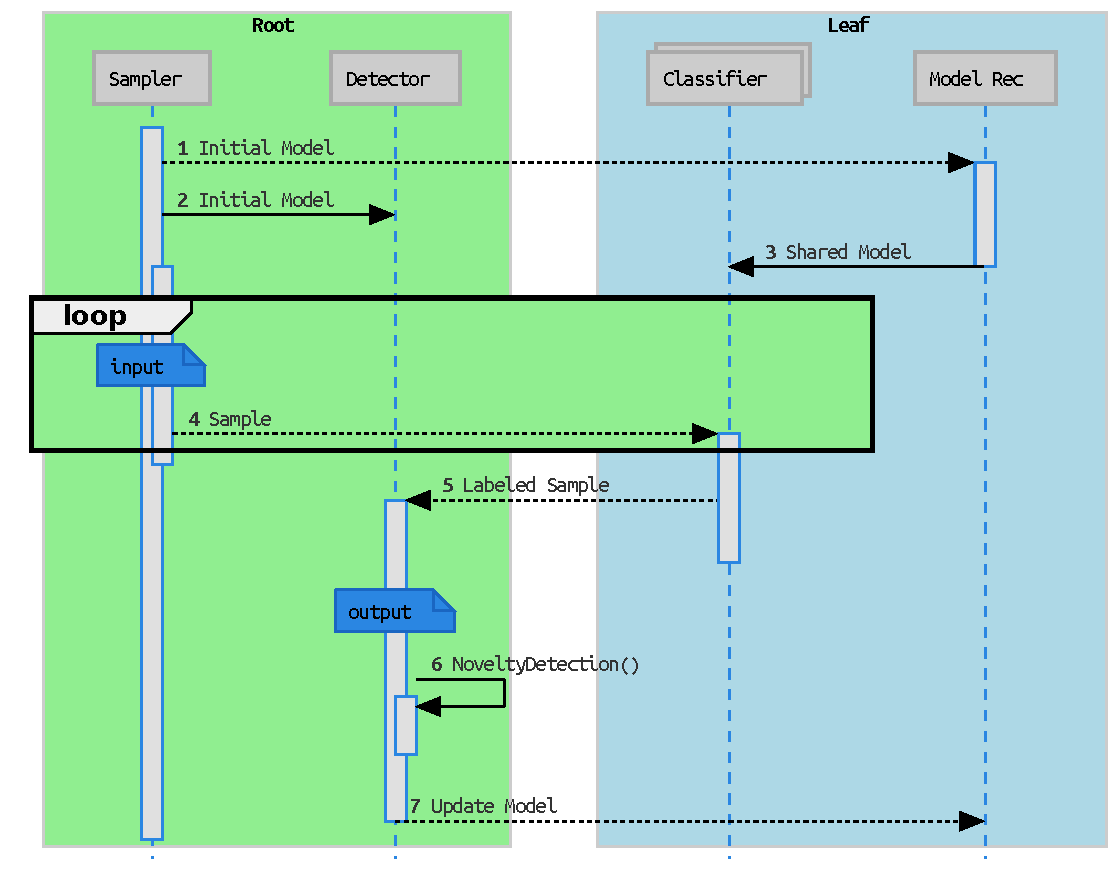
\includegraphics[width=0.80\linewidth,page=1]{figures/lifecycle-uml-svg.pdf}
  }
  \caption{Diagrama UML de Sequência do \mfog: visão geral das linhas de vida.}
  \label{fig:mfog-mpi-life}
\end{figure}

% For evaluation purposes, an \mfog implementation was made using MPI .
% The program is organized in a single program multiple data (SPMD)
% programming model, so a single version of the \mfog program was initiated on all
% nodes, being that one of them would perform the root role, while the others ran
% as leaves, the program entry point is illustrated on Algorithm \ref{alg:MFOG}.

% revisar aloritmo: Modelo? Trava? Que tal iniciar essas variáveis nas threads
% em cujo código elas são utilizadas? Como não são usadas aqui, acho que fica
% estranho...

\begin{algorithm}[htb]
    \SetKwFunction{nearestCluster}{clusterMaisPróximo}
    \SetKwFunction{clustering}{agrupamento}
    \SetKwFunction{NoveltyDetection}{DetecçãoNovidade}
    \SetKwFunction{handleModelSleep}{moveModeloAntigo}
    \SetKwFunction{removeOldSamples}{removeExemplosAntigos}
    % 
    \SetKwFunction{Mfog}{Mfog}
    \SetKwFunction{Sampler}{Fonte}
    \SetKwFunction{Classifier}{Classificador}
    \SetKwFunction{Detector}{Detector}
    \SetKwFunction{modelReceiver}{AtualizaModelo}
    % 
    \SetKwFunction{typeOf}{tipoDe}
    \SetKwFunction{Thread}{Thread}
    \SetKwFunction{Lock}{Trava}
    \SetKwFunction{readLock}{travaLeitura}
    \SetKwFunction{writeLock}{travaEscrita}
    % 
    \SetKwFunction{receive}{recebe}
    \SetKwFunction{send}{envia}
    \SetKwFunction{broadcast}{broadcast}
    % 
    \SetKwData{cleaningWindow}{janelaLimpeza}
    \SetKwData{noveltyDetectionTrigger}{gatilhoDetecçãoNovidade}
    \SetKwData{mpiSize}{mpiSize}
    \SetKwData{mpiRank}{mpiRank}
    \SetKwData{EndOfStream}{FimDeFluxo}
    % 
    \SetKwProg{Function}{Função}{:}{}
    \SetKw{continue}{continue}
    \SetKw{break}{pare}
    \SetKwFor{With}{com}{}{}
    % 
    \SetKwInOut{KwIn}{Entrada}
    \SetKwInOut{KwOut}{Saída}
    \SetKwInOut{KwParams}{Parâmetros}
    \KwParams{\mpiRank, \mpiSize}
    \KwIn{fluxoEntrada}
    \KwOut{fluxoSaída}
    % 
    \Function{\Mfog{fluxoEntrada, fluxoSaída}}{
        Modelo $\gets$ $\emptyset$; trava $\gets$ \textbf{new} \Lock()\; \label{line:init}
        \eIf(\emph{raiz}){\mpiRank == 0}{ \label{line:spmd}
            \textbf{new} \Thread(\Detector, [fluxoSaída, Modelo, trava])\;
            \Sampler(fluxoEntrada, Modelo, trava)\;
        }(\emph{folha}){
            \textbf{new} \Thread(\modelReceiver, [Modelo, trava])\;
            \Classifier(Modelo, trava)\;
        }
    }
\caption{Sistema M-FOG, ponto de entrada.}
\label{alg:MFOG}
\end{algorithm}

O Algoritmo \ref{alg:MFOG} mostra os primeiros passos do sistema \mfog, a
linha \ref{line:init} cria Modelo inicial como um conjunto vazio, e a trava
($lock$) utilizada para controle de acesso concorrente das \emph{threads}
\texttt{Detector} e \texttt{Fonte} no nó raiz e \texttt{AtualizaModelo} e
\texttt{Classificador} nos nós folha.

No processo raiz, de \texttt{mpiRank} $= 0$ e com acesso aos fluxos de entrada e
de saída, uma \emph{thread} com a função \texttt{Detector} é iniciada e a função
\texttt{Fonte} chamada.
Nos processos folha, de \texttt{mpiRank} $> 0$, uma \emph{thread} com a função
\texttt{AtualizaModelo} é iniciada e a função \texttt{Classificador} é chamada
pela \emph{thread} associada à função principal.

Destaca-se que a possibilidade de, ao invés de um \texttt{Classificador} por
processo e múltiplos processos por nó, pode-se utilizar um processo por nó
e múltiplas \emph{threads} executando \texttt{Classificador} por nó.
Esta estratégia economiza a transmissão de \mclusters para cada nó folha na
função \texttt{AtualizaModelo}, porém aumenta a concorrência de acesso ao modelo
entre as \emph{threads} executando \texttt{Classificador}.
Em avaliações simples comparando estas estratégias nenhum resultado conclusivo
foi observado e há espaço em trabalhos futuros para avaliações mais profundas
destas estratégias e outras de estratégias de otimização.

A função \texttt{Classificador}, listada no Algoritmo \ref{alg:MFOG-classifier}, é o
centro do sistema e opera com o modelo atualizado e um exemplo recebido como
mensagem do nó raiz.
Esta função calcula as distâncias entre o exemplo e todos \mclusters do modelo,
encontrando o mais próximo e verificando se o modelo explica aquele exemplo; se
explica, o rótulo do \mcluster mais próximo é atribuído como rótulo do exemplo.
A função \texttt{Classificador}, como as outras, só chega ao seu final se a
mensagem recebida (ou instância lida no caso da função \texttt{Fonte}) é um
marcador de fim de fluxo (\texttt{FimDeFluxo}, \emph{end of stream}, eos).

\begin{algorithm}[htb]
    \SetKwFunction{nearestCluster}{clusterMaisPróximo}
    \SetKwFunction{clustering}{agrupamento}
    \SetKwFunction{NoveltyDetection}{DetecçãoNovidade}
    \SetKwFunction{handleModelSleep}{moveModeloAntigo}
    \SetKwFunction{removeOldSamples}{removeExemplosAntigos}
    % 
    \SetKwFunction{Mfog}{Mfog}
    \SetKwFunction{Sampler}{Fonte}
    \SetKwFunction{Classifier}{Classificador}
    \SetKwFunction{Detector}{Detector}
    \SetKwFunction{modelReceiver}{AtualizaModelo}
    % 
    \SetKwFunction{typeOf}{tipoDe}
    \SetKwFunction{Thread}{Thread}
    \SetKwFunction{Lock}{Trava}
    \SetKwFunction{readLock}{travaLeitura}
    \SetKwFunction{writeLock}{travaEscrita}
    % 
    \SetKwFunction{receive}{recebe}
    \SetKwFunction{send}{envia}
    \SetKwFunction{broadcast}{broadcast}
    % 
    \SetKwData{cleaningWindow}{janelaLimpeza}
    \SetKwData{noveltyDetectionTrigger}{gatilhoDetecçãoNovidade}
    \SetKwData{mpiSize}{mpiSize}
    \SetKwData{mpiRank}{mpiRank}
    \SetKwData{EndOfStream}{FimDeFluxo}
    % 
    \SetKwProg{Function}{Função}{:}{}
    \SetKw{continue}{continue}
    \SetKw{break}{pare}
    \SetKwFor{With}{com}{}{}
    % 
    \SetKwInOut{KwIn}{Entrada}
    \SetKwInOut{KwOut}{Saída}
    \SetKwInOut{KwParams}{Parâmetros}
    % 
    \Function{\Classifier{Modelo, trava}}{
        \While{ Verdade }{
            exemplo $\gets$ \receive(TipoExemplo, raiz)\;
            \lIf{exemplo == \EndOfStream}{\break}
            exemplo.rótulo $\gets$ ``desconhecido''\;
            \With{\readLock(trava)}{
                (distância, cluster) $\gets$ \nearestCluster(exemplo, Modelo)\;
            }
            \If{distância $<$ cluster.raio}{
                exemplo.rótulo $\gets$ cluster.rótulo\;
            }
            \send(raiz, TipoExemplo, exemplo)\;
        }
    }
\caption{Função \texttt{Classificador} do nó folha do \mfog.}
\label{alg:MFOG-classifier}
\end{algorithm}

A função \texttt{AtualizaModelo}, listada no Algoritmo
\ref{alg:MFOG-model}, recebe novos \mclusters como mensagens do nó raiz,
independente deste \mcluster ser do modelo inicial, novidade ou extensão,
adequadamente travando o acesso ao modelo compartilhado com a \emph{thread}
executando a função \texttt{Classificador}.
Além da trava de acesso à leitura e escrita na implementação, a função
\texttt{Classificador} espera por um sinal emitido pela função
\texttt{AtualizaModelo}, indicando que o modelo está completo antes de começar a
busca pelo \mclusters mais próximo.

\begin{algorithm}[htb]
    \SetKwFunction{nearestCluster}{clusterMaisPróximo}
    \SetKwFunction{clustering}{agrupamento}
    \SetKwFunction{NoveltyDetection}{DetecçãoNovidade}
    \SetKwFunction{handleModelSleep}{moveModeloAntigo}
    \SetKwFunction{removeOldSamples}{removeExemplosAntigos}
    % 
    \SetKwFunction{Mfog}{Mfog}
    \SetKwFunction{Sampler}{Fonte}
    \SetKwFunction{Classifier}{Classificador}
    \SetKwFunction{Detector}{Detector}
    \SetKwFunction{modelReceiver}{AtualizaModelo}
    % 
    \SetKwFunction{typeOf}{tipoDe}
    \SetKwFunction{Thread}{Thread}
    \SetKwFunction{Lock}{Trava}
    \SetKwFunction{readLock}{travaLeitura}
    \SetKwFunction{writeLock}{travaEscrita}
    % 
    \SetKwFunction{receive}{recebe}
    \SetKwFunction{send}{envia}
    \SetKwFunction{broadcast}{broadcast}
    % 
    \SetKwData{cleaningWindow}{janelaLimpeza}
    \SetKwData{noveltyDetectionTrigger}{gatilhoDetecçãoNovidade}
    \SetKwData{mpiSize}{mpiSize}
    \SetKwData{mpiRank}{mpiRank}
    \SetKwData{EndOfStream}{FimDeFluxo}
    % 
    \SetKwProg{Function}{Função}{:}{}
    \SetKw{continue}{continue}
    \SetKw{break}{pare}
    \SetKwFor{With}{com}{}{}
    % 
    \SetKwInOut{KwIn}{Entrada}
    \SetKwInOut{KwOut}{Saída}
    \SetKwInOut{KwParams}{Parâmetros}
    \Function{\modelReceiver{Modelo, trava}}{
        \While{ Verdade }{
            cluster $\gets$ \receive(TipoCluster, raiz)\;
            \lIf{cluster == \EndOfStream}{\break}
            \With{\writeLock(trava)}{
                Modelo $\gets$ Modelo $\cup$ cluster\;
            }
        }
    }
\caption{Função \texttt{AtualizaModelo} do nó folha do \mfog.}
\label{alg:MFOG-model}
% \caption{Funções dos nós folha do \mfog: Atualização de Modelo e Classificador.}
% \label{alg:MFOG-leaf}
\end{algorithm}

A função \texttt{Fonte}, listada no Algoritmo \ref{alg:MFOG-sampler}, lê uma
instância do fluxo de entrada que pode ser do tipo exemplo ou do tipo \mcluster.
Se a instância for um exemplo, ele é enviado para um dos nós folha, o nó é
escolhido via balanceamento de carga \emph{round-robin}.
Se a instância for do tipo \mcluster, o modelo compartilhado com a \emph{thread}
executando a função \texttt{Detector} é travado para leitura e escrita e
atualizado, e o novo \mcluster é enviado para todas os nós folhas.

\begin{algorithm}[htb]
    \SetKwFunction{nearestCluster}{clusterMaisPróximo}
    \SetKwFunction{clustering}{agrupamento}
    \SetKwFunction{NoveltyDetection}{DetecçãoNovidade}
    \SetKwFunction{handleModelSleep}{moveModeloAntigo}
    \SetKwFunction{removeOldSamples}{removeExemplosAntigos}
    % 
    \SetKwFunction{Mfog}{Mfog}
    \SetKwFunction{Sampler}{Fonte}
    \SetKwFunction{Classifier}{Classificador}
    \SetKwFunction{Detector}{Detector}
    \SetKwFunction{modelReceiver}{AtualizaModelo}
    % 
    \SetKwFunction{typeOf}{tipoDe}
    \SetKwFunction{Thread}{Thread}
    \SetKwFunction{Lock}{Trava}
    \SetKwFunction{readLock}{travaLeitura}
    \SetKwFunction{writeLock}{travaEscrita}
    % 
    \SetKwFunction{receive}{recebe}
    \SetKwFunction{send}{envia}
    \SetKwFunction{broadcast}{broadcast}
    % 
    \SetKwData{cleaningWindow}{janelaLimpeza}
    \SetKwData{noveltyDetectionTrigger}{gatilhoDetecçãoNovidade}
    \SetKwData{mpiSize}{mpiSize}
    \SetKwData{mpiRank}{mpiRank}
    \SetKwData{EndOfStream}{FimDeFluxo}
    % 
    \SetKwProg{Function}{Função}{:}{}
    \SetKw{continue}{continue}
    \SetKw{break}{pare}
    \SetKwFor{With}{com}{}{}
    % 
    \SetKwInOut{KwIn}{Entrada}
    \SetKwInOut{KwOut}{Saída}
    \SetKwInOut{KwParams}{Parâmetros}
    \Function{\Sampler{fluxoEntrada, Modelo, trava}}{
        dest $\gets$ 1\;
        \ForEach{ {$exemplo_{i}$} $\in$ fluxoEntrada }{
            \If{\typeOf(exemplo) é TipoCluster}{
                \broadcast(TipoCluster, exemplo, raiz)\;
                \With{\writeLock(trava)}{
                    Modelo $\gets$ Modelo $\cup$ exemplo\;
                }
                \continue\;
            }
            % sample.label $\gets$ unknown\;
            \send(dest, TipoExemplo, exemplo)\;
            dest $\gets$ dest $+ 1$\;
            \lIf{dest $>$ \mpiSize}{dest $\gets$ 1}
        }
    }
\caption{Função \texttt{Fonte} do nó raiz do \mfog.}
\label{alg:MFOG-sampler}
\end{algorithm}

Enquanto a função \texttt{Fonte} gerencia a entrada de dados, a função
\texttt{Detector}, listada no Algoritmo \ref{alg:MFOG-detector}, gerencia a saída
de dados e, como tem acesso aos exemplos já classificados, também gerencia o
conjunto de desconhecidos.
Se o tamanho do conjunto de desconhecidos atinge um valor mínimo, a função de
detecção de novidade é chamada, os \mclusters representando padrões novidades ou
extensões são adicionados ao modelo e enviados para todos os nós folha.
Além da remoção dos exemplos utilizados para formar \mclusters de novidades e
extensões, exemplos que participaram duas vezes do processo de detecção de
novidade são considerados \emph{outliers} ou ruído e são removidos.

\begin{algorithm}[htb]
    \SetKwFunction{nearestCluster}{clusterMaisPróximo}
    \SetKwFunction{clustering}{agrupamento}
    \SetKwFunction{NoveltyDetection}{DetecçãoNovidade}
    \SetKwFunction{handleModelSleep}{moveModeloAntigo}
    \SetKwFunction{removeOldSamples}{removeExemplosAntigos}
    % 
    \SetKwFunction{Mfog}{Mfog}
    \SetKwFunction{Sampler}{Fonte}
    \SetKwFunction{Classifier}{Classificador}
    \SetKwFunction{Detector}{Detector}
    \SetKwFunction{modelReceiver}{AtualizaModelo}
    % 
    \SetKwFunction{typeOf}{tipoDe}
    \SetKwFunction{Thread}{Thread}
    \SetKwFunction{Lock}{Trava}
    \SetKwFunction{readLock}{travaLeitura}
    \SetKwFunction{writeLock}{travaEscrita}
    % 
    \SetKwFunction{receive}{recebe}
    \SetKwFunction{send}{envia}
    \SetKwFunction{broadcast}{broadcast}
    % 
    \SetKwData{cleaningWindow}{janelaLimpeza}
    \SetKwData{noveltyDetectionTrigger}{gatilhoDetecçãoNovidade}
    \SetKwData{mpiSize}{mpiSize}
    \SetKwData{mpiRank}{mpiRank}
    \SetKwData{EndOfStream}{FimDeFluxo}
    % 
    \SetKwProg{Function}{Função}{:}{}
    \SetKw{continue}{continue}
    \SetKw{break}{pare}
    \SetKwFor{With}{com}{}{}
    % 
    \SetKwInOut{KwIn}{Entrada}
    \SetKwInOut{KwOut}{Saída}
    \SetKwInOut{KwParams}{Parâmetros}
    \Function{\Detector{fluxoSaída, Modelo, trava}}{
        Desconhecidos $\gets \emptyset$;  últimaLimpeza $\gets 0$\;
        \While{ Verdade }{
            exemplo $\gets$ \receive(TipoExemplo, qualquer)\;
            \lIf{exemplo == \EndOfStream}{\break}
            % $out \gets$ exemplo\;
            fluxoSaída.adicione(exemplo)\;
            \If{exemplo.label == unknown}{
                Desconhecidos $\gets$ Desconhecidos $\cup$ exemplo\;
                \If{$|\;Desconhecidos\;| \geq$ \noveltyDetectionTrigger}{
                    novidades $\gets$ \NoveltyDetection(Modelo, *Desconhecidos)\;
                    \With{\writeLock(trava)}{
                        Modelo $\gets$ Modelo $\cup$ novidades\;
                    }
                    \ForEach{ cluster $\in$ novidades }{
                        \broadcast(TipoCluster, cluster, raiz)\;
                    }
                }
                \If{ exemplo.uid $ > $ ( últimaLimpeza $ + $ \cleaningWindow )}{
                    Desconhecidos $\gets$ \removeOldSamples(Desconhecidos, últimaLimpeza)\;
                    últimaLimpeza $ \gets $ exemplo.uid\;
                }
            }
        }
    }
\caption{Função \texttt{Detector} do nó raiz do \mfog.}
\label{alg:MFOG-detector}
% \caption{Funções do nó raiz do \mfog: Fonte e Detector.}
% \label{alg:MFOG-root}
\end{algorithm}

Em suma, a arquitetura do \mfog é composta de múltiplos nós numa névoa, que detectam
intrusão numa rede \iot. Para isso, os nós da rede processam de forma paralela e
distribuída o cálculo das distâncias e detecção de novidades, sendo assim um
sistema multiprocessado e distribuído. Utiliza-se um único programa com vários
processos por nó, e cada processo recebe um conjunto de dados diferentes
seguindo o paradigma \spmd.
